\subsection{Distributional Semantic Models in Practice}
\label{sec:dsm-in-practice}
\slidesrc{Distributional semantics (long version): 28--72}

The first part of the tutorial (Sections~\ref{sec:distributional-hypothesis}
to~\ref{sec:geometric-interpretation}) gave the idea: a word is a vector of counts, and
similar words have vectors pointing in similar directions. The long version of the deck
continues with what a real model looks like: how it is defined in general, how it is
built step by step, what we can do with it, three famous historical models, and a small
hands-on session.

This subsection covers:
\begin{enumerate}[nosep]
  \item the general definition of a distributional semantic model (DSM);
  \item the pipeline to build one, and the two kinds of co-occurrence matrix;
  \item what a DSM gives us: nearest neighbours, semantic maps, clusters, latent
        dimensions, word embeddings and context vectors;
  \item the difference between \emph{distributional} and \emph{distributed}
        representations;
  \item three famous models: LSA, Word Space and HAL;
  \item applications, software, and a toy laboratory in R.
\end{enumerate}

% ---------------------------------------------------------------------------
\subsubsection{General definition of DSMs}
\slidesrc{Distributional semantics (long version): 28--29}

In the hieroglyphs example (Section~\ref{sec:cooccurrence-matrix}) the cells of the
matrix were raw counts. Raw counts are rarely used as they are: very frequent contexts
(like the verb \emph{get}) dominate, and the numbers are very skewed (a few huge values,
many zeros). So a real model first \emph{rescales} or \emph{transforms} the counts.

\begin{nbdef}{Distributional semantic model (DSM)}
A \textbf{distributional semantic model} is a \textbf{scaled and/or transformed
co-occurrence matrix} $\mathbf{M}$, such that each row $\mathbf{x}$ represents the
distribution of a \textbf{target term} across contexts.

A \textbf{term} can be a word, a lemma, a phrase, a morpheme, a word pair, \ldots: any
unit whose meaning we want to represent.
\end{nbdef}

The slide shows the hieroglyphs matrix after such a transformation:

\begin{center}
\small
\begin{tabular}{@{}l rrrrrr@{}}
\toprule
 & \textbf{get} & \textbf{see} & \textbf{use} & \textbf{hear} & \textbf{eat} & \textbf{kill} \\
\midrule
knife  & 0.027 & $-0.024$ & 0.206 & $-0.022$ & $-0.044$ & $-0.042$ \\
cat    & 0.031 & 0.143 & $-0.243$ & $-0.015$ & $-0.009$ & 0.131 \\
\textcolor{nbred}{dog} & \textcolor{nbred}{$-0.026$} & \textcolor{nbred}{0.021} & \textcolor{nbred}{$-0.212$} & \textcolor{nbred}{0.064} & \textcolor{nbred}{0.013} & \textcolor{nbred}{0.014} \\
boat   & $-0.022$ & 0.009 & $-0.044$ & $-0.040$ & $-0.074$ & $-0.042$ \\
cup    & $-0.014$ & $-0.173$ & $-0.249$ & $-0.099$ & $-0.119$ & $-0.042$ \\
pig    & $-0.069$ & 0.094 & $-0.158$ & 0.000 & 0.094 & 0.265 \\
banana & 0.047 & $-0.139$ & $-0.104$ & $-0.022$ & 0.267 & $-0.042$ \\
\bottomrule
\end{tabular}
\captionof{table}{The hieroglyphs matrix after scaling: each row is still the vector of a
word, but the values are no longer counts.}
\end{center}

\begin{nbintuition}[why negative numbers?]
A count can never be negative, so these values cannot be counts. The slide does not say
which transformation was applied; negative values appear whenever we measure how much a
word occurs with a context \emph{compared to what we would expect by chance}. A positive
value says ``more often than expected'' (\emph{pig}--\emph{kill}: 0.265,
\emph{banana}--\emph{eat}: 0.267, \emph{knife}--\emph{use}: 0.206), a negative one ``less
often than expected'' (\emph{cat}--\emph{use}: $-0.243$: nobody \emph{uses} a cat).
Such ``association scores'' are much more informative than raw counts,
because a high raw count may only mean that both words are frequent.
\end{nbintuition}

% ---------------------------------------------------------------------------
\subsubsection{Building a distributional model}
\slidesrc{Distributional semantics (long version): 30--39}

Building a DSM is a pipeline of choices. Each box in Figure~\ref{fig:dsm-pipeline} is a
decision that changes the resulting model.

\begin{center}
\begin{tikzpicture}[
    box/.style={draw=nbblue, fill=nbblue!8, rounded corners=3pt, font=\small,
                inner sep=4pt, align=center, minimum height=0.7cm},
    lab/.style={font=\small, text=nbgreen!70!black},
    arr/.style={-{Stealth}, thick, nbblue},
    garr/.style={-{Stealth}, thick, nbgreen!70!black}]
  \node[box, draw=black, fill=black!6] (corpus) at (0,0)
        {pre-processed corpus with linguistic annotation};
  \node[box] (tt1) at (-3.3,-1.5) {define target terms};
  \node[box] (tt2) at (-3.3,-2.6) {context tokens or types};
  \node[box] (tf1) at (3.3,-1.5)  {define target \& feature terms};
  \node[box] (tf2) at (3.3,-2.6)  {type \& size of co-occurrence};
  \node[box, minimum width=0.9cm] (M) at (0,-3.6) {$\mathbf{M}$};
  \node[box] (fs) at (-2.6,-5.0) {feature scaling};
  \node[box] (sim) at (-2.6,-6.1) {similarity/distance measure + normalisation};
  \node[box] (dr) at (-2.6,-7.2) {dimensionality reduction};
  \draw[garr] (corpus.south) -- node[lab, above left] {term-context matrix} (tt1.north);
  \draw[garr] (corpus.south) -- node[lab, above right] {term-term matrix} (tf1.north);
  \draw[arr] (tt1) -- (tt2);
  \draw[arr] (tf1) -- (tf2);
  \draw[arr] (tt2.south) -- (M.north west);
  \draw[arr] (tf2.south) -- (M.north east);
  \draw[garr] (M.south) -- node[lab, above left] {geometric analysis} (fs.north);
  \draw[garr] (M.south) -- node[lab, above right] {probabilistic analysis} ++(2.8,-1.2);
  \draw[arr] (fs) -- (sim);
  \draw[arr] (sim) -- (dr);
\end{tikzpicture}
\captionof{figure}{The steps to build a distributional model.}
\label{fig:dsm-pipeline}
\end{center}

Step by step:
\begin{enumerate}
  \item \textbf{Pre-processed corpus with linguistic annotation.} We start from a large
        corpus that has been segmented into words
        (Section~\ref{sec:word-segmentation}), often lemmatised
        (Section~\ref{sec:stemming-lemmatization}), POS-tagged
        (Section~\ref{sec:pos-tagging}) and sometimes parsed. The annotation lets us
        count, e.g., ``\emph{dog} as object of \emph{see}'' instead of just ``\emph{dog}
        near \emph{see}''.
  \item \textbf{Choose the kind of matrix.} Two families:
        \begin{itemize}[nosep]
          \item a \textbf{term-term matrix}: rows are target terms, columns are other
                terms (\textbf{feature terms}). We must define both sets and decide the
                \textbf{type and size of co-occurrence}: ``within a window of 5 words'',
                ``in the same sentence'', ``as verb and its object'', \ldots
          \item a \textbf{term-context matrix}: rows are target terms, columns are
                \textbf{contexts} such as sentences, documents, Web pages or encyclopaedia
                articles. We decide whether the columns are context \textbf{tokens} (each
                single document is a column) or context \textbf{types} (similar
                contexts grouped together).
        \end{itemize}
  \item \textbf{The matrix $\mathbf{M}$} is filled with counts.
  \item \textbf{Analysis.} It can be \emph{probabilistic} (the counts are seen as
        probabilities of co-occurrence) or, as in this course, \emph{geometric}
        (treat the rows as vectors). The geometric branch has three further choices:
        \begin{itemize}[nosep]
          \item \textbf{feature scaling}: how to rescale the counts: logarithm,
                weights similar to TF-IDF, association scores (see the warning in
                Section~\ref{sec:cooccurrence-matrix});
          \item \textbf{similarity/distance measure + normalisation}: e.g.\ cosine
                similarity, or vectors normalised to length 1
                (Section~\ref{sec:geometric-interpretation});
          \item \textbf{dimensionality reduction}: compress thousands of columns into a
                few hundred (e.g.\ with SVD, see below).
        \end{itemize}
\end{enumerate}

\begin{nbexample}{a term-term matrix and a term-context matrix}
\textbf{Term-term matrix}: how often each target term co-occurs with each feature term
(a dash means 0):
\begin{center}
\small
\begin{tabular}{@{}l rrrrrrr@{}}
\toprule
 & breed & tail & feed & kill & important & explain & likely \\
\midrule
cat    & 83  & 17 & 7   & 37  & --  & 1   & --  \\
dog    & 561 & 13 & 30  & 60  & 1   & 2   & 4   \\
animal & 42  & 10 & 109 & 134 & 13  & 5   & 5   \\
time   & 19  & 9  & 29  & 117 & 81  & 34  & 109 \\
reason & 1   & -- & 2   & 14  & 68  & 140 & 47  \\
cause  & --  & 1  & --  & 4   & 55  & 34  & 55  \\
effect & --  & -- & 1   & 6   & 60  & 35  & 17  \\
\bottomrule
\end{tabular}
\end{center}
\textbf{Term-context matrix}: how often each term occurs in each context (here, each
column is one Wikipedia-like article):
\begin{center}
\small
\begin{tabular}{@{}l rrrrrrr@{}}
\toprule
 & Felidae & Pet & Feral & Bloat & Philosophy & Kant & Back pain \\
\midrule
cat    & 10 & 10 & 7  & -- & -- & -- & -- \\
dog    & -- & 10 & 4  & 11 & -- & -- & -- \\
animal & 2  & 15 & 10 & 2  & -- & -- & -- \\
time   & 1  & -- & -- & -- & 2  & 1  & -- \\
reason & -- & 1  & -- & -- & 1  & 4  & 1  \\
cause  & -- & -- & -- & 2  & 1  & 2  & 6  \\
effect & -- & -- & -- & 1  & -- & 1  & -- \\
\bottomrule
\end{tabular}
\end{center}
In both matrices the words split into two groups. \emph{cat}, \emph{dog},
\emph{animal} co-occur with \emph{breed}, \emph{tail}, \emph{feed} and appear in the
articles about pets; \emph{reason}, \emph{cause}, \emph{effect} co-occur with
\emph{important}, \emph{explain}, \emph{likely} and appear in the articles about
philosophy and medicine. \emph{Time} sits in between: it co-occurs with almost
everything, as very general words do.
\end{nbexample}

\begin{nbwarning}[term-term vs.\ term-context]
Do not mix them up. In a \textbf{term-term} matrix the columns are \emph{words}, so the
matrix tells us which words appear \emph{near} which words. In a \textbf{term-context}
matrix the columns are \emph{pieces of text} (documents, sentences), so it tells us in
\emph{which texts} a word appears. The second is the classic matrix of information
retrieval: transposed, its columns are the TF-IDF document vectors of
Section~\ref{sec:stop-words-tfidf}.
\end{nbwarning}

% ---------------------------------------------------------------------------
\subsubsection{What a DSM gives us}
\slidesrc{Distributional semantics (long version): 40--50}

Once every word is a vector, many things become simple geometry.

\paragraph{Nearest neighbours.}
Take a DSM built from verb--object relations in the British National Corpus (BNC),
reduced to 100 dimensions with SVD. For a word, list the other words whose vectors form
the smallest \textbf{angle} with it (the angle is the ``cosine angle''
$\alpha = \arccos(\cos\alpha)$ of Section~\ref{sec:geometric-interpretation}, in
degrees: small angle = very similar):

\begin{center}
\small
\begin{tabularx}{\linewidth}{@{}l X@{}}
\toprule
\textbf{target} & \textbf{nearest neighbours (angle in degrees)} \\
\midrule
\emph{trousers} & shirt (18.5), blouse (21.9), scarf (23.4), jeans (24.7), skirt (25.9),
  sock (26.2), shorts (26.3), jacket (27.8), glove (28.1), coat (28.8), cloak (28.9),
  hat (29.1), tunic (29.3), overcoat (29.4), pants (29.8), helmet (30.4), apron (30.5),
  robe (30.6), mask (30.8), tracksuit (31.0), jersey (31.6), shawl (31.6), \ldots \\
\emph{rage} & anger (28.5), fury (32.5), sadness (37.0), disgust (37.4), emotion (39.0),
  jealousy (40.0), grief (40.4), irritation (40.7), revulsion (40.7), scorn (40.7),
  panic (40.8), bitterness (41.6), resentment (41.8), indignation (41.9),
  excitement (42.0), hatred (42.5), envy (42.8), disappointment (42.9), \ldots \\
\bottomrule
\end{tabularx}
\end{center}
All neighbours of \emph{trousers} are clothes, all neighbours of \emph{rage} are
emotions, and the closest ones are near-synonyms (\emph{anger}, \emph{fury}). The model
was never told what clothes or emotions are: it only saw which verbs take these nouns as
objects (\emph{wear}, \emph{put on}, \emph{take off} for clothes; \emph{feel},
\emph{express}, \emph{hide} for emotions).

\begin{nbexample}{reading an angle}
$\alpha = 18.5^\circ$ for \emph{trousers}--\emph{shirt} means
$\cos\alpha = \cos 18.5^\circ \approx 0.948$: the two vectors point in almost the same
direction. $\alpha = 28.5^\circ$ for \emph{rage}--\emph{anger} gives
$\cos\alpha \approx 0.879$. Angles are easier to read than cosines because they spread
the values out: $0.948$ and $0.879$ look close, $18.5^\circ$ and $28.5^\circ$ do not.
\end{nbexample}

\paragraph{Similarity graph.}
The neighbours can be drawn as a graph: one node per word, an edge between two words when
they are close (small angle). The graph of the neighbours of \emph{trousers} is a dense
web of clothes, with \emph{trousers} and \emph{shirt} at its centre; the graph of
\emph{plant} is more interesting, because \emph{plant} is ambiguous: its neighbours form
\textbf{two groups}, one for the industrial plant (factory, station, reactor, mill,
brewery, smelter, laboratory, \ldots) and one for the living plant (crop, species,
flower, seed, seedling, shrub, \ldots).

\begin{center}
\begin{tikzpicture}[w/.style={font=\small, inner sep=1.5pt},
    e/.style={nbblue!45, thin}]
  \node[w, text=nbred, font=\small\bfseries] (p) at (0,0) {plant};
  % industrial sense
  \foreach \n/\x/\y in {factory/-2.6/0.9, station/-3.4/0.1, reactor/-2.9/-0.8,
      mill/-1.8/-1.2, brewery/-4.2/-0.9, smelter/-4.4/0.8, laboratory/-1.7/1.4,
      machinery/-3.6/1.6}
     \node[w] (\n) at (\x,\y) {\n};
  % living sense
  \foreach \n/\x/\y in {crop/2.0/0.9, species/2.9/0.1, flower/2.4/-0.9, seed/1.6/-1.3,
      seedling/3.9/-0.8, shrub/4.0/0.8, tree/2.8/1.6}
     \node[w] (\n) at (\x,\y) {\n};
  \foreach \a/\b in {p/factory,p/station,p/reactor,p/mill,p/laboratory,factory/station,
      factory/mill,station/reactor,reactor/smelter,mill/brewery,brewery/smelter,
      factory/machinery,machinery/smelter,station/smelter,laboratory/factory,reactor/mill}
     \draw[e] (\a) -- (\b);
  \foreach \a/\b in {p/crop,p/species,p/flower,p/seed,crop/species,crop/tree,species/shrub,
      flower/seed,flower/seedling,seed/seedling,shrub/seedling,tree/shrub,species/flower}
     \draw[e] (\a) -- (\b);
  \node[font=\footnotesize\itshape, text=nbgray] at (-3.0,-1.8) {plant = factory};
  \node[font=\footnotesize\itshape, text=nbgray] at (3.0,-1.8) {plant = living thing};
\end{tikzpicture}
\captionof{figure}{Similarity graph of the neighbours of \emph{plant} (redrawn and
simplified; the word \emph{tree} is added for readability). The two senses of the word
show up as two clusters joined only through \emph{plant} itself.}
\end{center}

\begin{nbwhy}[distributional semantics meets word senses]
The vector of an ambiguous word is a \emph{mixture} of its senses: \emph{plant} is
partly near factories and partly near flowers. Looking at how its neighbours cluster is
a way to discover the senses automatically (\emph{word sense induction}), without a
dictionary like WordNet (Section~\ref{sec:wordnet}).
\end{nbwhy}

\paragraph{Semantic maps.}
Vectors have hundreds of dimensions, but they can be projected onto a plane so that close
vectors stay close. The slide shows 44 concrete nouns of six categories (birds, ground
animals, green vegetables, fruit, tools, vehicles), from the same verb--object DSM:

\begin{center}
\begin{tikzpicture}
\begin{axis}[width=11cm, height=9cm, xmin=-1.8, xmax=2.0, ymin=-1.6, ymax=1.5,
    title={Semantic map (V--Obj from BNC), redrawn approximately},
    title style={font=\small}, tick label style={font=\scriptsize},
    legend style={font=\scriptsize, at={(1.02,1)}, anchor=north west},
    nodes near coords, point meta=explicit symbolic,
    every node near coord/.append style={font=\tiny, anchor=south west, inner sep=1pt}]
  \addplot[only marks, mark=*, mark size=2pt, nbred] coordinates {
    (-0.72,0.55)[chicken] (-0.75,-0.60)[eagle] (-0.75,-0.10)[duck] (-0.60,-0.22)[swan]
    (-1.16,-0.42)[owl] (-1.63,0.0)[penguin] (-0.84,-0.89)[peacock]};
  \addlegendentry{bird}
  \addplot[only marks, mark=*, mark size=2pt, nbgray!60!yellow] coordinates {
    (-0.35,-0.12)[dog] (-0.95,-0.35)[elephant] (-0.30,-0.30)[cow] (-0.50,0.03)[cat]
    (-0.50,-0.47)[lion] (-0.98,-0.07)[pig] (-0.43,0.23)[snail] (-1.40,-1.05)[turtle]};
  \addlegendentry{groundAnimal}
  \addplot[only marks, mark=*, mark size=2pt, nbgreen] coordinates {
    (-0.62,1.33)[mushroom] (-0.24,0.44)[corn] (-0.20,0.60)[lettuce] (-0.30,1.14)[potato]
    (-0.15,1.28)[onion]};
  \addlegendentry{green}
  \addplot[only marks, mark=*, mark size=2pt, nbteal!50!cyan] coordinates {
    (-0.12,0.38)[cherry] (-0.59,1.18)[banana] (-0.32,0.69)[pear] (-0.72,0.71)[pineapple]};
  \addlegendentry{fruitTree}
  \addplot[only marks, mark=*, mark size=2pt, nbblue] coordinates {
    (1.29,0.56)[bottle] (1.14,0.05)[pencil] (1.31,0.16)[pen] (1.09,1.23)[cup]
    (0.74,0.84)[bowl] (1.44,-0.55)[scissors] (1.00,0.69)[kettle] (1.45,-0.07)[knife]
    (1.71,-0.65)[screwdriver] (0.81,-0.51)[hammer] (0.85,0.16)[spoon] (0.74,-0.38)[chisel]
    (0.87,-0.30)[telephone]};
  \addlegendentry{tool}
  \addplot[only marks, mark=*, mark size=2pt, nbpurple] coordinates {
    (0.05,-0.68)[boat] (0.41,-1.32)[car] (-0.24,-0.97)[ship] (0.31,-1.13)[truck]
    (0.16,-0.54)[rocket] (-0.04,-0.44)[motorcycle] (-0.15,-1.44)[helicopter]};
  \addlegendentry{vehicle}
\end{axis}
\end{tikzpicture}
\captionof{figure}{A semantic map: each noun is a point, colours are the true
categories (not used by the model). Tools on the right, vehicles at the bottom, food at
the top, animals on the left.}
\end{center}

The categories come out as regions of the plane, even though the model never saw them.
The borders are not perfect: \emph{chicken} sits next to the fruit and vegetables, which
makes sense from the point of view of verbs (we \emph{eat} and \emph{cook} chicken).

\paragraph{Clustering.}
A clustering algorithm groups the vectors automatically. With \emph{hierarchical}
clustering we get a \textbf{dendrogram}: a tree whose leaves are the words; two branches
join at a height that measures how different the two groups are (high joins = very
different groups).

\begin{center}
\begin{tikzpicture}[x=1cm, y=0.09cm, leaf/.style={font=\scriptsize, align=center,
    anchor=north, text width=2.2cm}]
  % leaves (groups) at y=20
  \node[leaf] at (0,18) {kettle, cup, bottle, bowl, hammer, knife, spoon, pencil, pen,
     chisel, scissors, screwdriver, telephone};
  \node[leaf] at (2.4,18) {motorcycle, rocket, car, truck, helicopter, boat, ship};
  \node[leaf] at (4.8,18) {peacock, eagle, lion};
  \node[leaf] at (7.2,18) {pineapple, mushroom, onion, cherry, pear, corn,
     \textcolor{nbred}{chicken}, potato, banana, lettuce};
  \node[leaf] at (9.6,18) {turtle, penguin, swan, owl, snail, duck, elephant, dog, cat,
     cow, pig};
  % groups merged inside (vertical lines from 20 up to their internal height)
  \draw[thick, nbblue] (0,20) -- (0,55);
  \draw[thick, nbpurple] (2.4,20) -- (2.4,60);
  \draw[thick, nbred] (4.8,20) -- (4.8,68);
  \draw[thick, nbgreen] (7.2,20) -- (7.2,58);
  \draw[thick, nbgray] (9.6,20) -- (9.6,63);
  % merges
  \draw[thick] (0,55) -- (0,82) -- (2.4,82) -- (2.4,60);
  \draw[thick] (4.8,68) -- (4.8,74) -- (7.2,74) -- (7.2,58);
  \draw[thick] (6.0,74) -- (6.0,86) -- (9.6,86) -- (9.6,63);
  \draw[thick] (1.2,82) -- (1.2,92) -- (7.8,92) -- (7.8,86);
  % axis
  \draw[-{Stealth}] (-1.6,20) -- (-1.6,96) node[above, font=\scriptsize] {cluster size};
  \foreach \v in {20,40,60,80} \draw (-1.65,\v) -- (-1.55,\v) node[left, font=\tiny] {\v};
\end{tikzpicture}
\captionof{figure}{Hierarchical clustering of the 44 concrete nouns (redrawn and
simplified: each leaf here is a group of words that the original dendrogram joins
low). The vertical axis is the dissimilarity at which groups merge.}
\end{center}

Artefacts (tools, vehicles) separate from natural things (food, animals) at the top.
The clustering is good but not perfect: \emph{chicken} goes with food, and
\emph{peacock}, \emph{eagle}, \emph{lion} form a small group of their own (they are
mostly \emph{seen}, rarely \emph{eaten} or \emph{fed}). These ``errors'' are informative:
they show that the model captures how words are \emph{used}, not a biological taxonomy.

\paragraph{Latent dimensions.}
Plot the nouns using only two columns of the matrix: how often each noun is the object
of \emph{buy} ($x$ axis) and of \emph{sell} ($y$ axis), on a log scale.

\begin{center}
\begin{tikzpicture}
\begin{axis}[width=8.5cm, height=7.5cm, xmin=0, xmax=4.6, ymin=0, ymax=4.6,
    xlabel={buy}, ylabel={sell}, tick label style={font=\scriptsize},
    label style={font=\small}, nodes near coords, point meta=explicit symbolic,
    every node near coord/.append style={font=\tiny, anchor=west, inner sep=1pt}]
  \addplot[only marks, mark=*, mark size=1pt, black] coordinates {
    (0.1,3.6)[liquor] (0.5,2.6)[advertising] (1.8,2.75)[insurance] (4.0,4.05)[share]
    (3.7,4.38)[good] (3.4,4.15)[copy] (4.0,3.3)[house] (3.6,3.6)[land] (2.9,3.4)[asset]
    (2.9,3.0)[stock] (3.4,2.7)[book] (3.6,2.1)[food] (3.0,1.95)[drink] (1.4,0.7)[time]
    (1.2,1.0)[year] (2.6,0.5)[suit] (3.4,1.3)[pair] (0.7,1.4)[system] (0.8,2.1)[arm]
    (1.2,2.0)[work] (2.2,1.9)[property] (2.5,1.4)[ticket]};
  \draw[-{Stealth}, very thick, nbred] (axis cs:0,0) -- (axis cs:4.1,4.1);
  \node[font=\scriptsize, text=nbred, rotate=45] at (axis cs:1.85,1.3) {latent dimension};
\end{axis}
\end{tikzpicture}
\captionof{figure}{Nouns by how often they are bought and sold (redrawn approximately,
a few words only). The red arrow is the direction along which most words lie.}
\end{center}

Most words lie along the diagonal: things that are bought are also sold. So the two
columns \emph{buy} and \emph{sell} are largely \emph{redundant}; together they really
measure one underlying (\textbf{latent}) property, ``being an object of commercial
transactions''. A single axis along the red arrow describes these words almost as well
as the two original axes. This is exactly what \textbf{dimensionality reduction} does on
the whole matrix: it finds a few latent dimensions that summarise many correlated
columns.

\begin{nbintuition}[SVD in one paragraph]
The \textbf{singular value decomposition} (SVD) is the standard tool for this. It rotates
the coordinate system so that the first new axis follows the direction of largest
spread of the points (the red arrow), the second axis the largest remaining spread, and
so on. Keeping only the first $k$ new axes (e.g.\ $k = 100$ or 300) gives short vectors
that keep most of the information, remove noise, and make similar words closer (two
synonyms that never share an exact context may still share a latent dimension).
\end{nbintuition}

\paragraph{Word embeddings and context vectors.}
A DSM vector is a \textbf{sub-symbolic} representation of meaning: no single number
means anything to a human (unlike a dictionary definition or a WordNet synset), but the
vector as a whole encodes how the word is used. Such vectors are used as
\begin{itemize}[nosep]
  \item a \textbf{feature vector} for a machine learning algorithm;
  \item the \textbf{input of a neural network}.
\end{itemize}

They can also represent a \emph{single occurrence} of a word in context.
\textbf{Context vectors} (Schütze, 1998) use a \textbf{bag-of-words} approach: the
vector of a sentence is the \textbf{centroid} (the average) of the vectors of all the
context words in it. This can be applied to word sense disambiguation (WSD,
Section~\ref{sec:word-sense-disambiguation}).

\begin{center}
\begin{tikzpicture}[scale=1.25, v/.style={-{Stealth}, thin}]
  \draw[-{Stealth}, thick] (0,0) -- (4.2,0) node[below left, font=\small\bfseries] {animals};
  \draw[-{Stealth}, thick] (0,0) -- (0,3.9) node[above, rotate=90, anchor=south east,
       font=\small\bfseries] {computers};
  \draw[v] (0,0) -- (0.3,3.6) node[above, font=\scriptsize] {computer};
  \draw[v] (0,0) -- (1.0,2.9) node[right, font=\scriptsize] {keyboard};
  \draw[v] (0,0) -- (1.3,2.1) node[right, font=\scriptsize] {connect};
  \draw[v] (0,0) -- (2.9,1.6) node[right, font=\scriptsize] {furry};
  \draw[v] (0,0) -- (3.1,0.8) node[right, font=\scriptsize] {cat};
  \draw[v] (0,0) -- (2.2,0.35) node[right, font=\scriptsize] {chase};
  \draw[-{Stealth}, very thick, nbgreen] (0,0) -- (0.87,2.87);
  \draw[-{Stealth}, very thick, nbblue] (0,0) -- (2.73,0.92);
  \node[font=\scriptsize, text=nbgreen!70!black, align=left, anchor=west] at (1.5,3.5)
       {``connect the \textbf{mouse} and\\ keyboard to the computer''};
  \node[font=\scriptsize, text=nbblue, align=left, anchor=west] at (3.4,1.25)
       {``the furry cat chased\\ the \textbf{mouse}''};
\end{tikzpicture}
\captionof{figure}{Context vectors in a toy 2-dimensional space. Each thin arrow is a
word vector; each thick arrow is the centroid of the context words of a sentence. The two
occurrences of \emph{mouse} get very different context vectors.}
\label{fig:context-vectors}
\end{center}

\begin{nbexample}{disambiguating \emph{mouse}}
With the toy vectors of Figure~\ref{fig:context-vectors}, the first sentence has context
words \emph{connect}, \emph{keyboard}, \emph{computer}:
\[
  \tfrac{1}{3}\bigl[(1.3, 2.1) + (1.0, 2.9) + (0.3, 3.6)\bigr]
  = \tfrac{1}{3}(2.6,\ 8.6) \approx (0.87,\ 2.87),
\]
pointing towards ``computers''. The second has \emph{furry}, \emph{cat}, \emph{chase}:
\[
  \tfrac{1}{3}\bigl[(2.9, 1.6) + (3.1, 0.8) + (2.2, 0.35)\bigr]
  = \tfrac{1}{3}(8.2,\ 2.75) \approx (2.73,\ 0.92),
\]
pointing towards ``animals''. Comparing each context vector (with the cosine) to
prototype vectors of the two senses, we pick the device in the first sentence and the
rodent in the second: this is WSD without any dictionary. (The numbers are invented for
the picture; real vectors have hundreds of dimensions.)
\end{nbexample}

% ---------------------------------------------------------------------------
\subsubsection{Distributional vs.\ distributed}
\slidesrc{Distributional semantics (long version): 51--53}

Two words that sound alike and are often confused:

\begin{center}
\small
\begin{tabularx}{\linewidth}{@{}>{\raggedright\arraybackslash}X >{\raggedright\arraybackslash}X@{}}
\toprule
\textbf{Distributional model} & \textbf{Distributed representation} \\
\midrule
captures the linguistic \emph{distribution} of each word as a high-dimensional numeric
vector &
a \emph{sub-symbolic} representation of words as high-dimensional numeric vectors \\
typically (but not necessarily) based on co-occurrence counts &
similarity of vectors usually (but not necessarily) corresponds to semantic similarity
of the words \\
relies on the distributional hypothesis: distributional similarity $\sim$ semantic
similarity &
hot topic: unsupervised neural \textbf{word embeddings} (word2vec, GloVe, \ldots) \\
\bottomrule
\end{tabularx}
\end{center}

\begin{nbfact}{the relation between the two}
\emph{Distributional} says where the vector comes from (the contexts of the word);
\emph{distributed} says what the vector is (meaning spread over many numbers, none of
which is meaningful alone). A distributional model \textbf{can be used as} a distributed
representation, and neural word embeddings are both.
\end{nbfact}

% ---------------------------------------------------------------------------
\subsubsection{Three famous examples}
\slidesrc{Distributional semantics (long version): 54--61}

Three historical models follow. Each one is a different set of choices in the
pipeline of Figure~\ref{fig:dsm-pipeline}.

\paragraph{Latent Semantic Analysis (LSA; Landauer and Dumais, 1997).}
\begin{itemize}[nosep]
  \item Corpus: 30\,473 articles of Grolier's Academic American Encyclopedia (4.6
        million words), each article cut to its first 2\,000 characters.
  \item A \textbf{word-article} (term-context) frequency matrix for 60\,768 words: the row
        of a word gives its frequency in each article.
  \item Scaling: logarithmic frequencies, scaled by the \textbf{entropy} of the word
        (a word spread evenly over all articles has high entropy and says little about
        any of them, so it gets a low weight; the same idea as the idf).
  \item Reduced to 300 dimensions by \textbf{SVD}, a technique borrowed from Latent
        Semantic Indexing (LSI, Dumais et al., 1988) in information retrieval. Central
        claim: SVD reveals \emph{latent semantic features}, it is not just a data
        reduction technique.
  \item Evaluation: the \textbf{TOEFL synonym test} (80 items: given a word, choose its
        synonym among four options). LSA got \textbf{64.4\%} correct, about the score of
        non-native applicants to US universities. The authors also simulated the learning
        rate of vocabulary based on the TOEFL results.
\end{itemize}

\paragraph{Word Space (Schütze, 1992, 1993, 1998).}
\begin{itemize}[nosep]
  \item Corpus: about 60 million words of news messages from the New York Times News
        Service.
  \item A \textbf{word-word} (term-term) co-occurrence matrix: 20\,000 target words and
        2\,000 context words as features. The row records how often each context word
        occurs \emph{close to} the target word, in a window of 50 words left and right
        (1998) or about 1\,000 characters (1992).
  \item Rows weighted by inverse document frequency (tf.idf).
  \item \textbf{Context vector} = centroid of the word vectors of a context
        (bag-of-words, Figure~\ref{fig:context-vectors}); goal: determine the
        ``meaning'' of a context.
  \item Reduced to 100 SVD dimensions, mainly for efficiency.
  \item Evaluation: \textbf{unsupervised word sense induction} by clustering the
        context vectors of an ambiguous word; the induced senses improve information
        retrieval performance.
\end{itemize}

\paragraph{HAL (Hyperspace Analogue to Language; Lund and Burgess, 1996).}
\begin{itemize}[nosep]
  \item Corpus: 160 million words from newsgroup postings.
  \item A \textbf{word-word} matrix where the same 70\,000 words are both targets and
        features; co-occurrence window of 1 to 10 words.
  \item \textbf{Separate counts for left and right co-occurrence}: \emph{the} before
        \emph{dog} and \emph{the} after \emph{dog} are different features, so the
        context is \emph{structured}. In later work co-occurrences are weighted by
        (inverse) distance: a word right next to the target counts more than one ten
        words away (Li et al., 2000).
  \item No dimensionality reduction.
  \item Applications include semantic vocabulary maps, obtained by
        \textbf{multidimensional scaling} (MDS) to 2 dimensions (a projection that
        tries to keep the distances between points).
\end{itemize}

\begin{center}
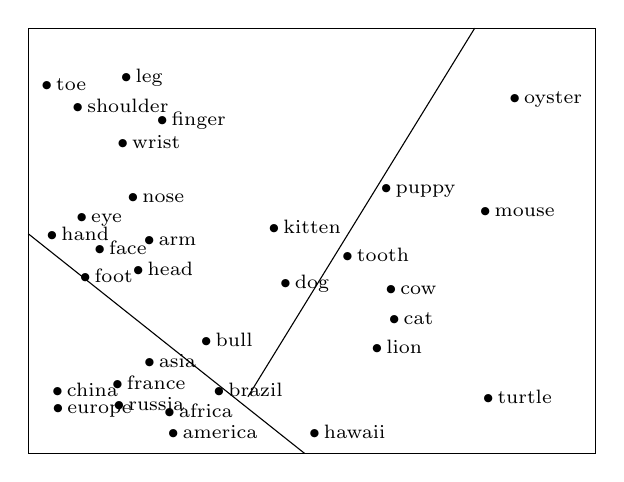
\begin{tikzpicture}[scale=0.9, w/.style={font=\scriptsize}]
  \draw (0,0) rectangle (8,6);
  \draw (0,3.1) -- (3.9,0);
  \draw (3.1,0.8) -- (6.3,6);
  \foreach \n/\x/\y in {toe/0.5/5.2, leg/1.6/5.3, shoulder/1.3/4.9, finger/2.3/4.7,
      wrist/1.7/4.4, nose/1.8/3.6, eye/1.0/3.3, hand/0.7/3.1, face/1.3/2.9, arm/2.0/3.0,
      foot/1.1/2.5, head/1.9/2.6}
     \node[w] at (\x,\y) {$\bullet$\,\n};
  \foreach \n/\x/\y in {puppy/5.5/3.7, kitten/3.9/3.2, mouse/6.9/3.4, tooth/4.9/2.8,
      dog/3.9/2.4, cow/5.4/2.3, cat/5.4/1.9, bull/2.8/1.6, lion/5.2/1.5, oyster/7.3/5.0,
      turtle/6.9/0.8}
     \node[w] at (\x,\y) {$\bullet$\,\n};
  \foreach \n/\x/\y in {china/0.8/0.9, europe/0.9/0.6, france/1.7/1.0, russia/1.7/0.7,
      asia/2.0/1.3, africa/2.4/0.6, america/2.6/0.3, brazil/3.1/0.9, hawaii/4.5/0.3}
     \node[w] at (\x,\y) {$\bullet$\,\n};
\end{tikzpicture}
\captionof{figure}{A HAL vocabulary map obtained by multidimensional scaling (redrawn
approximately): body parts at the top left, places at the bottom, animals on the right.
The two lines separate the three regions.}
\end{center}

\begin{center}
\small
\begin{tabularx}{\linewidth}{@{}l >{\raggedright\arraybackslash}X >{\raggedright\arraybackslash}X >{\raggedright\arraybackslash}X@{}}
\toprule
 & \textbf{LSA} & \textbf{Word Space} & \textbf{HAL} \\
\midrule
matrix & term-context (word $\times$ article) & term-term, window 50 words & term-term,
  window 1--10, left/right separate \\
corpus & encyclopaedia, 4.6M words & news, 60M words & newsgroups, 160M words \\
scaling & log + entropy & tf.idf & (later) inverse distance \\
reduction & SVD, 300 dim. & SVD, 100 dim. & none \\
evaluation & TOEFL synonyms (64.4\%) & word sense induction & semantic maps (MDS) \\
\bottomrule
\end{tabularx}
\captionof{table}{The three famous DSMs side by side.}
\end{center}

\begin{nbfact}{many parameters}
There is an enormous range of DSM parameters and applications: the three examples are
three entirely different models, each tuned to its own application. So we need an
overview of the parameters and of their effects (the further parts of the tutorial: the
parameters of a DSM, evaluating DSM representations, the mathematics of DSMs,
understanding distributional semantics). The lesson: \textbf{distributional semantics is
an empirical science}: which choices work best is found by experiment, not derived from
first principles.
\end{nbfact}

% ---------------------------------------------------------------------------
\subsubsection{Applications and software}
\slidesrc{Distributional semantics (long version): 62--66}

Some applications of DSMs in computational linguistics:
\begin{itemize}[nosep]
  \item unsupervised part-of-speech induction (Schütze, 1995): words with similar
        distributions tend to have the same POS;
  \item word sense disambiguation (Schütze, 1998);
  \item query expansion in information retrieval (Grefenstette, 1994): add to a query
        the nearest neighbours of its words;
  \item synonym tasks and other language tests (Landauer and Dumais, 1997; Turney et
        al., 2003);
  \item thesaurus compilation (Lin, 1998; Rapp, 2004);
  \item ontology and wordnet expansion (Pantel et al., 2009);
  \item attachment disambiguation (Pantel and Lin, 2000): in ``eat pizza with a fork''
        does \emph{with a fork} attach to \emph{eat} or to \emph{pizza}?
  \item probabilistic language models (Bengio et al., 2003), the ancestor of neural
        language models;
  \item sub-symbolic input representation for neural networks;
  \item many other tasks in computational semantics: entailment detection, noun compound
        interpretation, identification of non-compositional expressions (idioms such as
        \emph{kick the bucket}), \ldots
\end{itemize}

The field had many dedicated workshops between 2007 and 2014 (CoSMo, GeMS, DiSCo, CVSC,
ESSLLI courses, \ldots). Software packages:

\begin{center}
\small
\begin{tabularx}{\linewidth}{@{}l l X@{}}
\toprule
\textbf{package} & \textbf{language} & \textbf{notes} \\
\midrule
HiDEx & C++ & re-implementation of the HAL model \\
SemanticVectors & Java & scalable architecture based on random indexing \\
S-Space & Java & complex object-oriented framework \\
JoBimText & Java & UIMA / Hadoop framework \\
Gensim & Python & complex framework, focus on parallelisation and out-of-core algorithms
  (it also implements word2vec) \\
DISSECT & Python & user-friendly, designed for research on compositional semantics \\
wordspace & R & interactive research laboratory, but scales to real-life data sets \\
\bottomrule
\end{tabularx}
\end{center}

Further material: the wordspace wiki (\url{http://wordspace.collocations.de/}), the open
source tutorial, and the review paper by Turney and Pantel (2010), \emph{From frequency
to meaning: Vector space models of semantics}, Journal of Artificial Intelligence
Research 37, 141--188.

% ---------------------------------------------------------------------------
\subsubsection{R as a toy laboratory}
\slidesrc{Distributional semantics (long version): 67--72}

The tutorial uses the statistical environment \textbf{R} (with RStudio and the CRAN
packages \texttt{sparsesvd} and \texttt{wordspace}) as a laboratory. The
\texttt{wordspace} package contains the matrices seen above as example data sets: the
hieroglyphs matrix, the term-term matrix and the term-context matrix (each stored under a
name such as \texttt{DSM\_HieroglyphsMatrix}). The basic operations on a DSM matrix:

\begin{minted}{r}
library(wordspace)
# apply log-transformation to de-skew co-occurrence frequencies
M <- log2(DSM_HieroglyphsMatrix + 1)
round(M, 3)
# compute semantic distance (cosine similarity)
pair.distances("dog", "cat", M, convert=FALSE)
#   dog/cat
# 0.9610952
# find nearest neighbours
nearest.neighbours(M, "dog", n=3)
#      cat      pig      cup
# 16.03458 20.08826 31.77784
plot(nearest.neighbours(M, "dog", n=3, dist.matrix=TRUE))
\end{minted}

What each line does:
\begin{itemize}[nosep]
  \item \texttt{log2(M + 1)} replaces each count $f$ by $\log_2(1+f)$: the scaling step
        of the pipeline. The ``$+1$'' avoids $\log 0$ (a zero count stays 0).
  \item \texttt{pair.distances(\ldots, convert=FALSE)} returns the cosine similarity
        itself; it is 0.961, the value of the hieroglyphs slide
        (Section~\ref{sec:cooccurrence-matrix}). This confirms how that value was
        computed.
  \item \texttt{nearest.neighbours} returns the closest words with their
        \emph{angles} in degrees: $\arccos(0.961) \approx 16.0^\circ$ for \emph{cat},
        $20.1^\circ$ for \emph{pig}, $31.8^\circ$ for \emph{cup}.
\end{itemize}

\begin{nbexercise}{\thesubsection.1}{from cosine to angle and back}
Using the log-scaled hieroglyphs matrix, $\cos(\text{dog}, \text{pig}) = 0.939$ and
$\cos(\text{dog}, \text{cup}) = 0.850$ (Section~\ref{sec:cooccurrence-matrix}).
(a) Compute the corresponding angles. (b) Why does \emph{cup} come third among the
neighbours of \emph{dog} although it is not an animal?
\end{nbexercise}
\begin{nbsolution}
(a) $\alpha = \arccos(0.939) \approx 20.1^\circ$ and $\alpha = \arccos(0.850) \approx
31.8^\circ$, the values printed by \texttt{nearest.neighbours}.

(b) With only six contexts the model is very coarse. \emph{Cup} and \emph{dog} are both
very frequent objects of \emph{get} and \emph{see}, and after the log scaling these two
columns weigh a lot. The contexts that would separate them (\emph{hear}, \emph{eat},
\emph{kill}) are only three. With thousands of contexts, as in a real DSM, \emph{cup}
would be far from \emph{dog}. Lesson: the quality of a DSM depends on how many and which
contexts are used.
\end{nbsolution}

\begin{nbsummary}[DSMs in practice]
\begin{itemize}[nosep]
  \item DSM = scaled and/or transformed co-occurrence matrix; each row represents a
        target term (word, lemma, phrase, \ldots).
  \item Pipeline: annotated corpus $\to$ term-term matrix (targets, features, type and
        size of co-occurrence) or term-context matrix (targets, context tokens/types)
        $\to$ $\mathbf{M}$ $\to$ feature scaling $\to$ similarity measure +
        normalisation $\to$ dimensionality reduction.
  \item Uses: nearest neighbours (angles), similarity graphs (ambiguous words split
        into clusters), semantic maps, clustering, latent dimensions (SVD), features for
        ML, context vectors (centroids) for WSD.
  \item Distributional (where the vector comes from) vs.\ distributed (sub-symbolic
        vector); a DSM can be used as a distributed representation.
  \item LSA: word $\times$ article, log + entropy, SVD 300, TOEFL 64.4\%. Word Space:
        word $\times$ word, window 50, tf.idf, SVD 100, sense induction. HAL: word
        $\times$ word, left/right counts, no reduction, MDS maps.
  \item Distributional semantics is an empirical science.
\end{itemize}
\end{nbsummary}
